% Définition du répertoire contenant les images
\graphicspath{{IMAGE/}}

% FRAME Intro
\begin{frame}


\includegraphics[width=12cm]{Logos.pdf}

\vfill

\begin{center}

\vspace*{1.5cm}

\LARGE
\textbf{Concentration, Segregation, Autocorrelation}

\vspace*{1.5cm}
 DELHI GIS-R School


\large
9-12\up{th} April 2019

\vspace*{1.5cm}


\textbf{Hadrien Commenges \& Paul Chapron}

{\small

\vspace*{0.1cm}

\url{hadrien.commenges@univ-paris1.fr}

\url{paul.chapron@ign.fr}
}

\end{center}

\end{frame}

% FRAME
\begin{frame}{A good starting point}

\textbf{Information about tools and methods }

~

GeoDa Center for Geospatial Analysis and Computation (Luc Anselin)

\url{https://geodacenter.asu.edu}

~

$\rightarrow$ logiciels \emph{standalone} (GeoDa) + Python and  R libraries \\
$\rightarrow$ tutorials, references, online courses


\end{frame}


% FRAME
\begin{frame}{Concentration}

\textbf{Classical methods from inequality economics}

\begin{figure}
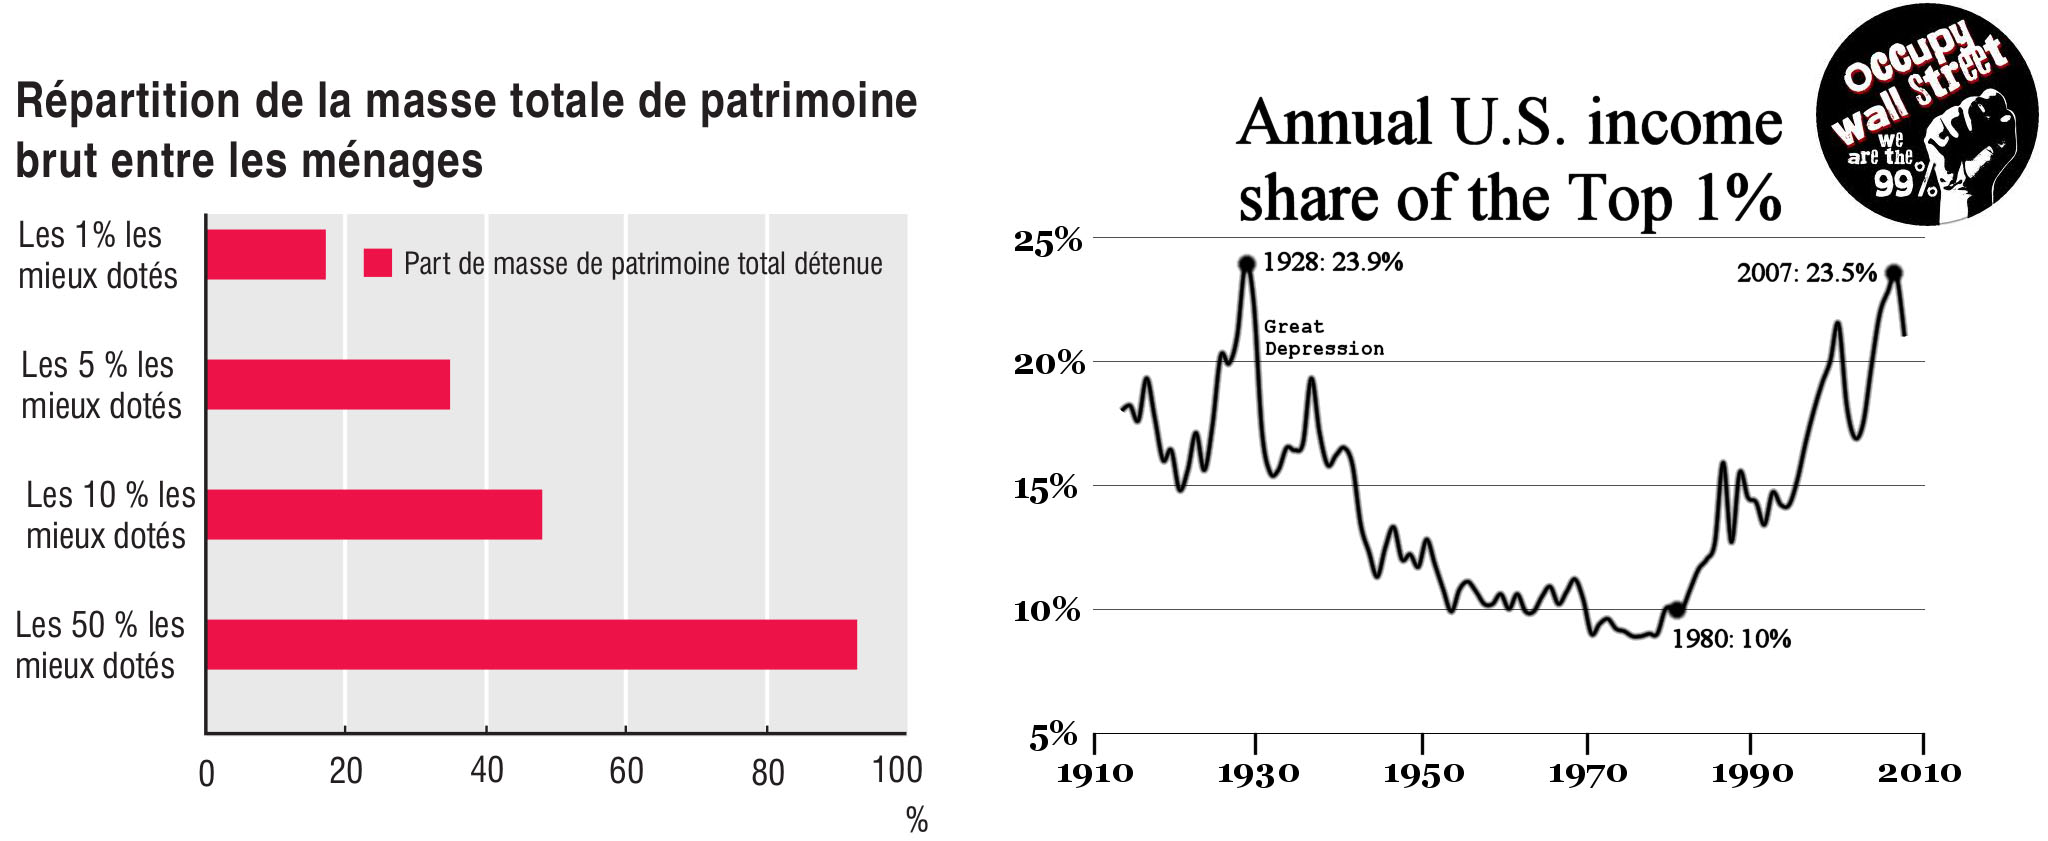
\includegraphics[width=12cm]{Inequalities.jpg}
\end{figure}

\end{frame}


% FRAME
\begin{frame}{Concentration}

\textbf{Hoover  index} \\
\emph{(Dissimilarity index} or \emph{Duncan's I)}

~

For two classes $x$ and $y$ of a population  that sum up to 100\% (e.g. male / female), 

\begin{equation}
\nonumber
H = \frac{1}{2} \sum_{i=1}^n \bigg| \frac{x_i}{x_{tot}} - \frac{y_i}{y_{tot}} \bigg|
\end{equation}


(also the longest vertical distance between the lorenz Curve and the 45 degrees line of perfect equality)

\end{frame}


% FRAME
\begin{frame}{Concentration}
\begin{figure}
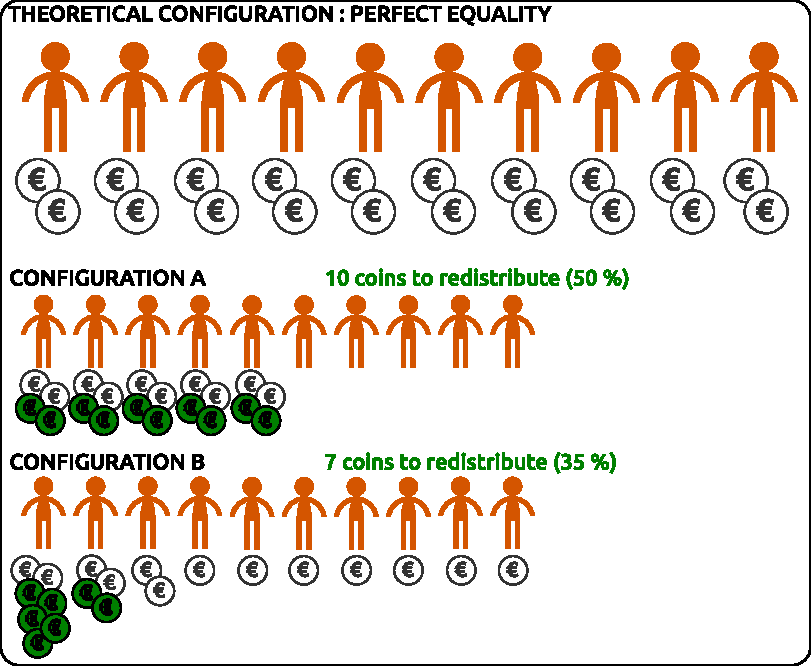
\includegraphics[width=9cm]{Gateau2_EN.pdf}
\end{figure}

\end{frame}



% FRAME
\begin{frame}{Concentration}

\textbf{Gini index}

~

relative mean of absolute differences between every pair of a stock 

\begin{equation}
\nonumber
G = \frac{\sum_i \sum_j |x_i - x_j|}{2n \sum_i x_i}
\end{equation}


ranges from 0 (perfect equality) to 1 (perfect inequality), but these theoretical values are never reached.





\end{frame}	



% FRAME
\begin{frame}{Concentration}


%TODO figure EN 
\begin{figure}
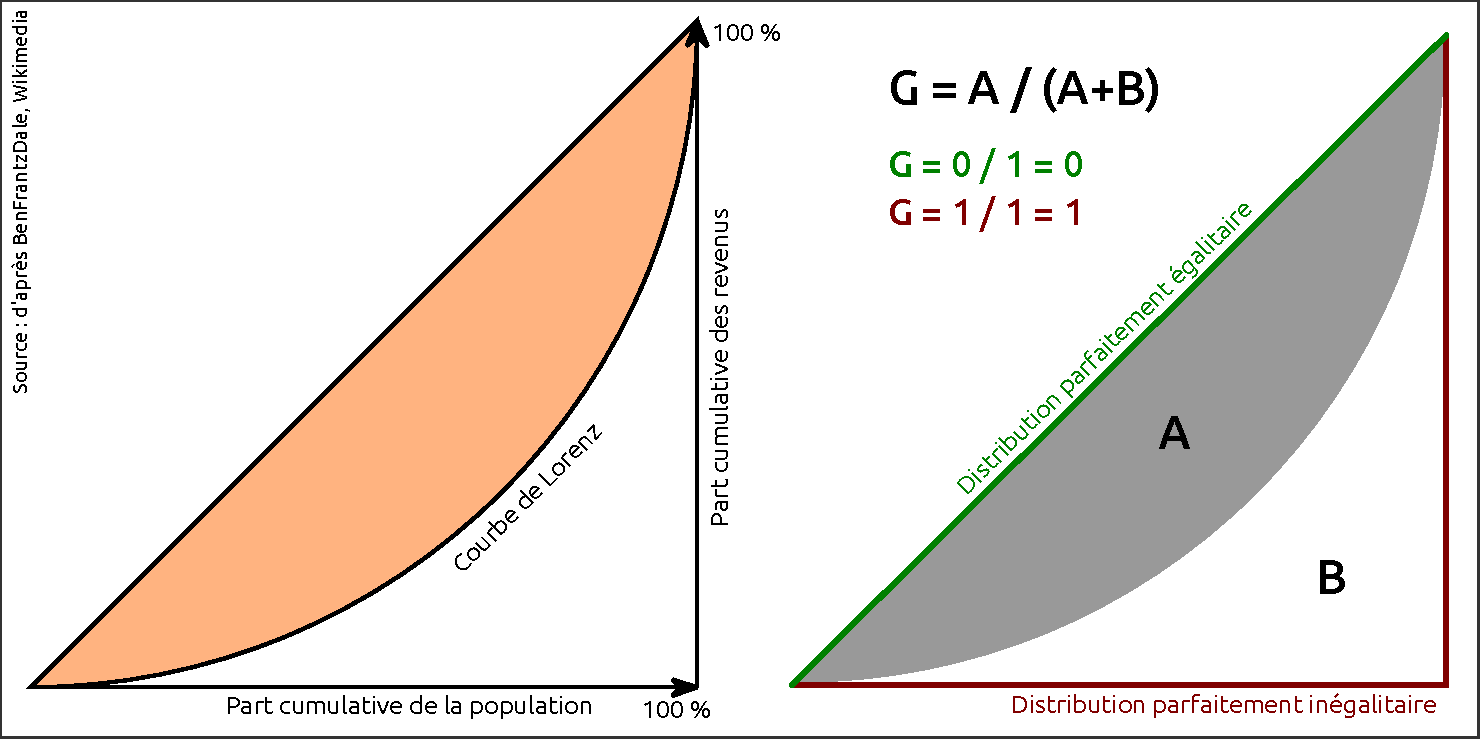
\includegraphics[width=12cm]{Lorenz.pdf}
\end{figure}

\end{frame}


% FRAME
\begin{frame}{Segregation}

\textbf{Entropy-based measures}

These meassures comes from the field of information theory (Shannon) ~

\textbf{Quantity of information $I$ (in bits) of a message $m$ :} logarithm (base 2) of the ratio between the finite set of every possible message before a message is recieved ($M$, the universe) and  the finite set of possible message after it is recieved ($m$):

~

\begin{equation}
\nonumber
  I = \log\left(\frac{M}{m} \right) = - \log(p(m))
\end{equation}

~

This quantity is expressed in \emph{bits} since the logarithm base is 2.

\end{frame}


% FRAME
\begin{frame}{Segregation}

\textbf{Entropy-based measures}

~ 

\textbf{I}: Information brought by the occcurence of a message (informative event) . 

\textbf{H} (entropy): information stored in a finite set of informative event (e.g. all the messages of a transmission) \\ 
- i.e. average quantity of information stored in a set of messages \\ 
- i.e. each message bring as much information as its quantity of information multiplied by its probability of apparition.

\begin{equation}
  H(x) = - \sum\limits_{i=1}^n p_i \log(p_i)
  \nonumber
\end{equation}

~

\textbf{Relative entropy:} ratio between an entropy and the maximum entropy $H_{max}$

\begin{equation}
  H_{max} = \log(n)
  \nonumber
\end{equation}

\end{frame}



% FRAME
\begin{frame}{Segregation}

\textbf{Entropy interpretation guide}

~ 

Low (relative) entropy values tend to indicate segregated configurations

~

High (relative) entropy values tend to indicate more evenly distributed configurations



\end{frame}



% FRAME
\begin{frame}{Autocorrelation}

Hoover, Gini, Shannon (Theil) indexes can't distinguish between these configurations \\ 

\begin{figure}
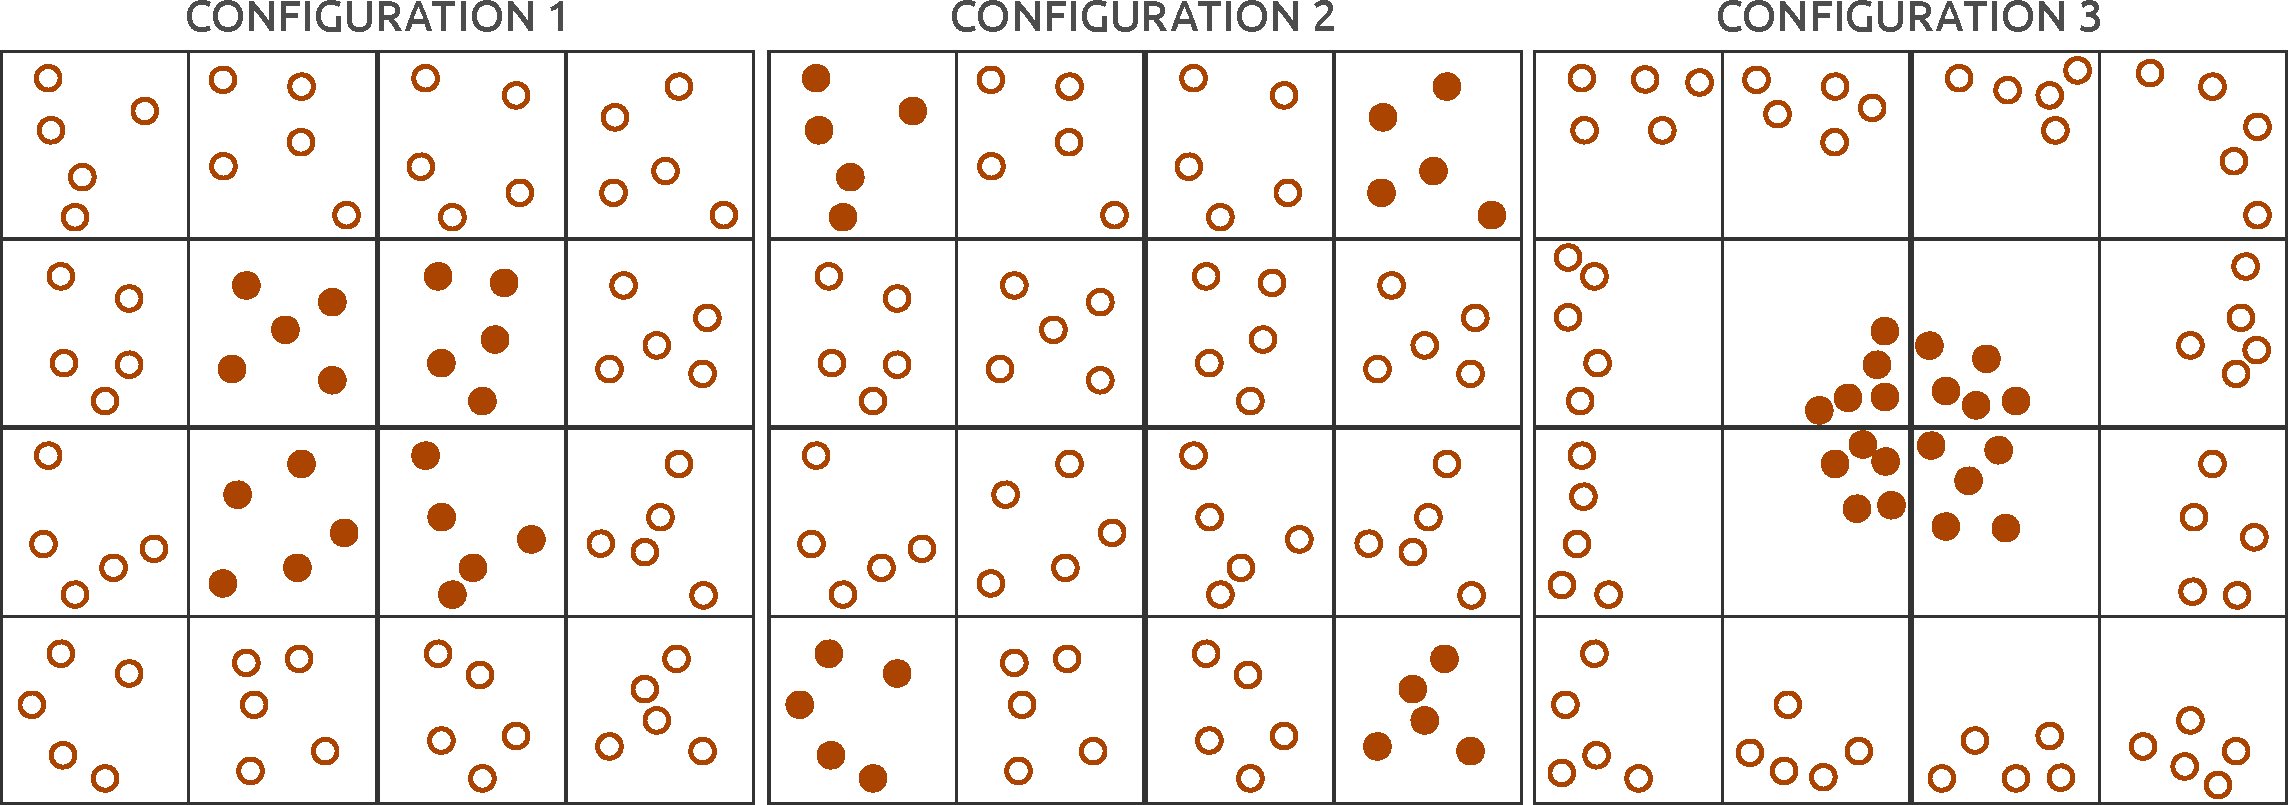
\includegraphics[width=12cm]{NonSpatial.pdf}
\end{figure}

Autocorrelation indexes (\textbf{Geary} and \textbf{Moran}) can distinguish between \textbf{1} et \textbf{2}.

\end{frame}


% FRAME
\begin{frame}{Autocorrelation}

Moran's I (1950):

$$
I = \frac{n}{\sum_{i} \sum_{j} w_{ij}} \times \frac{\sum_{i} \sum_{j} w_{ij} (x_i - \bar{x})(x_j - \bar{x})}{\sum_{i} (x_i - \bar{x})^2}
$$

~

$n$ : number of spatial units \\ 
$x_i$ et $x_j$ : values of $x$ in $i$ and $j$ \\ 
$\bar{x}$ : average value of $x$ \\ 
$w_{ij}$ : weighting matrix corresponding to the neighborhood definition

\end{frame}



% FRAME
\begin{frame}{Autocorrelation}

\textbf{Moran's I} interpretation based on \textbf{Moran's plot}

\begin{figure}
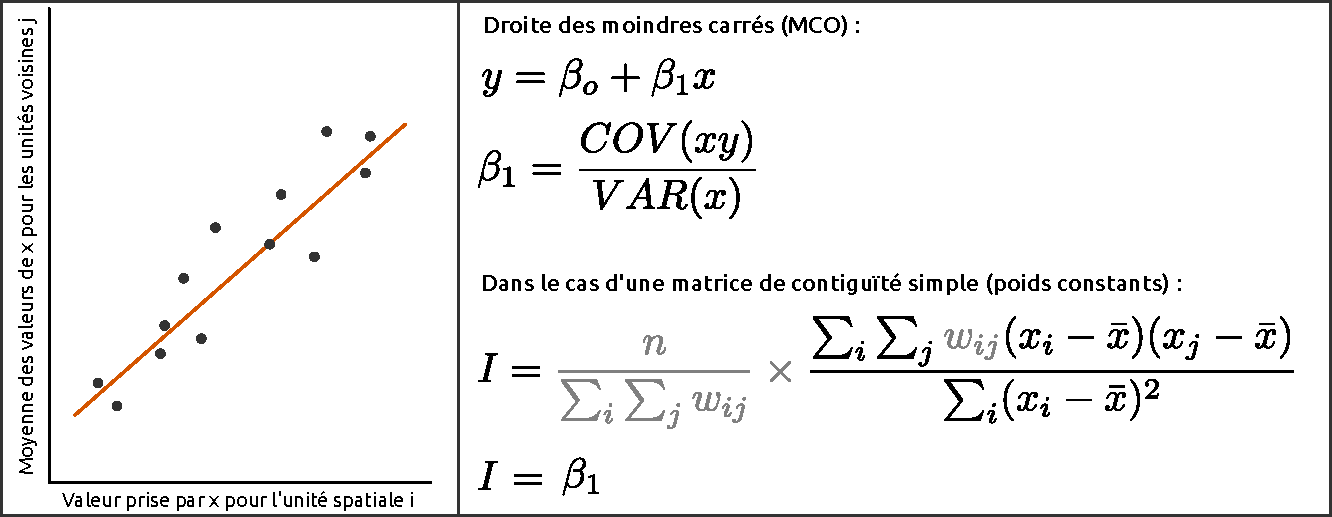
\includegraphics[width=12cm]{MoranPlot.pdf}
\end{figure}

\end{frame}


% FRAME
\begin{frame}{Autocorrelation}

\textbf{Local contribution to the global autocorrelation index} \\
LISA - \emph{local indicators of spatial autocorrelation}

$$
I_i = z_i \sum_{j} w_{ij} z_j
$$

~

$z_i$ standardized value of $x$ for spatial unit $i$ \\
$z_j$ standardized value of $x$ for spatial unit $j$ \\
$w_{ij}$ weighting matrix

\end{frame}


% FRAME
\begin{frame}{Spatial autoregressive model}

The autocorrelation can be used in a \textbf{descriptive} approach or in a \textbf{modeling} approach.

~

Ex. of land values modeling (econometrics): the value of a dwelling is function of:

\begin{itemize}
  \item Intrinsic attributes: surface area, garden, etc.
  \item Contextual attributes: i.e. the value of the dwellings in the neighborhood
\end{itemize}

~

In this case, it may be useful to build a \textbf{spatial autoregressive regression} (SAR), i.e. to inject the \textbf{lagged values} (neighborhood average) as a regressor.

\end{frame}


